\documentclass[aspectratio=169]{beamer}
\usepackage[utf8]{inputenc}
\usepackage[T5]{fontenc}
\usepackage[vietnamese]{babel}
\usepackage{graphicx}
\usepackage{hyperref}
\usepackage{lmodern}

% Theme
\usetheme{Madrid}
\usecolortheme{whale}

% Metadata
\title[AI \& ML trong NN]{Thu Hoạch Trí Tuệ: AI và ML Cách Mạng Hóa Nông Nghiệp}
\subtitle{Chương 7}
\author{Giảng viên}
\institute{Đại học Đông Á}
\date{\today}

\begin{document}

\begin{frame}
    \titlepage
\end{frame}

\begin{frame}{Nội dung chính}
    \tableofcontents
\end{frame}

\section{Giới thiệu chung}
\begin{frame}{Giới thiệu chung}
    \begin{itemize}
        \item Nông nghiệp là xương sống của nền văn minh nhân loại, hiện đang trải qua sự thay đổi lớn nhờ công nghệ.
        \item \textbf{Học máy (Machine Learning - ML)} đóng vai trò then chốt:
        \begin{itemize}
            \item Xử lý khối lượng lớn dữ liệu.
            \item Trích xuất những hiểu biết có ý nghĩa.
            \item Nâng cao năng suất, tính bền vững và hiệu quả tổng thể.
        \end{itemize}
    \end{itemize}
\end{frame}

\section{Dự đoán năng suất}
\begin{frame}{Dự đoán năng suất cây trồng}
    ML giúp tận dụng dữ liệu lịch sử và dữ liệu thời gian thực để ước tính chính xác năng suất trong tương lai.
    \begin{figure}[h]
        \centering
        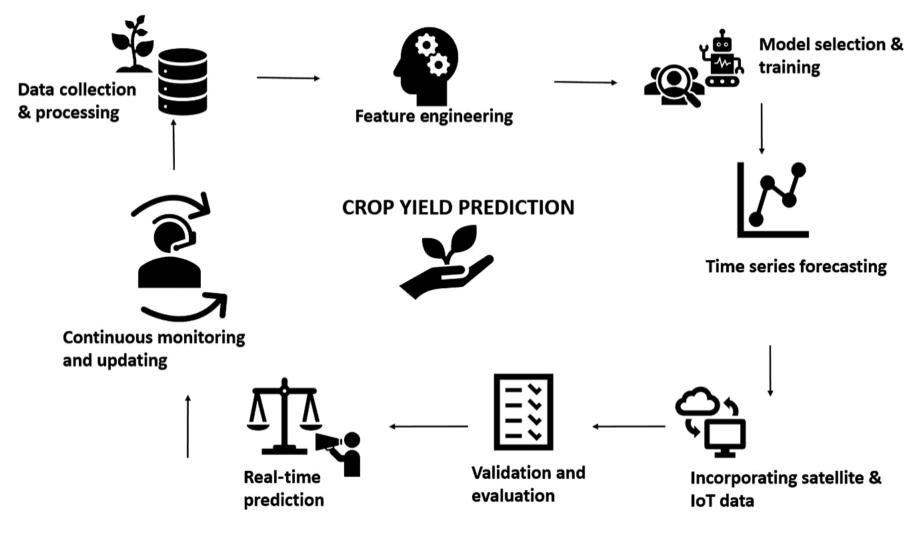
\includegraphics[height=0.6\textheight]{images/chap7_p2_1.jpeg}
        \caption{Hình 7.1: Sơ đồ dự đoán năng suất cây trồng bằng ML}
    \end{figure}
\end{frame}

\begin{frame}{Các bước dự đoán năng suất cây trồng}
    \begin{enumerate}
        \item \textbf{Thu thập và tiền xử lý dữ liệu}: Làm sạch dữ liệu, xử lý giá trị thiếu và ngoại lai.
        \item \textbf{Kỹ thuật đặc trưng}: Trích xuất các yếu tố liên quan như nhiệt độ, lượng mưa, độ ẩm, phân bón.
        \item \textbf{Lựa chọn \& Huấn luyện mô hình}: Sử dụng Hồi quy tuyến tính, SVM, Mạng nơ-ron, LSTM...
        \item \textbf{Xác thực và đánh giá}: Tinh chỉnh và kiểm định chéo để tăng khả năng tổng quát.
        \item \textbf{Dự đoán thời gian thực}: Áp dụng mô hình dựa trên điều kiện thời tiết hiện tại.
    \end{enumerate}
\end{frame}

\section{Quản lý dịch hại}
\begin{frame}{Phát hiện bệnh và Quản lý dịch hại}
    Tận dụng \textbf{Thị giác máy tính} và phân tích hình ảnh để xác định nhanh chóng các bệnh và sâu bệnh:
    \begin{itemize}
        \item \textbf{Thu thập \& Tiền xử lý}: Chụp ảnh độ phân giải cao từ Drone/Vệ tinh, loại bỏ nhiễu.
        \item \textbf{Phân đoạn \& Trích xuất}: Phân đoạn vùng lá bệnh, trích xuất màu sắc, kết cấu.
        \item \textbf{Phân loại \& Nhận dạng}: Sử dụng mạng nơ-ron tích chập (CNN) để phân biệt cây khỏe và cây nhiễm bệnh.
        \item \textbf{Giám sát sớm}: Cảnh báo trước khi dịch bệnh lây lan rộng.
    \end{itemize}
\end{frame}

\section{Sức khỏe đất}
\begin{frame}{Sức khỏe đất và Quản lý dinh dưỡng}
    Phân tích độ phì nhiêu của đất bằng ML để tối ưu hóa dinh dưỡng:
    \begin{itemize}
        \item \textbf{Thu thập mẫu}: Thu thập mẫu từ nhiều vị trí (loại đất, pH, nitơ, phốt pho, kali).
        \item \textbf{Lựa chọn đặc trưng \& Mô hình}: Sử dụng Cây quyết định, Rừng ngẫu nhiên, GBM.
        \item \textbf{Huấn luyện \& Đánh giá}: Tìm kiếm lưới (Grid Search) để tối ưu hóa siêu tham số, đánh giá bằng RMSE, R-squared.
        \item \textbf{Triển khai}: Người dùng nhập dữ liệu đất và nhận dự đoán độ phì nhiêu để lên kế hoạch bón phân hợp lý.
    \end{itemize}
\end{frame}

\section{Tối ưu hóa tưới tiêu}
\begin{frame}{Tối ưu hóa tưới tiêu: Mạng cảm biến}
    Việc triển khai các mạng cảm biến là cốt lõi để giám sát độ ẩm đất và điều kiện thời tiết:
    \begin{figure}[h]
        \centering
        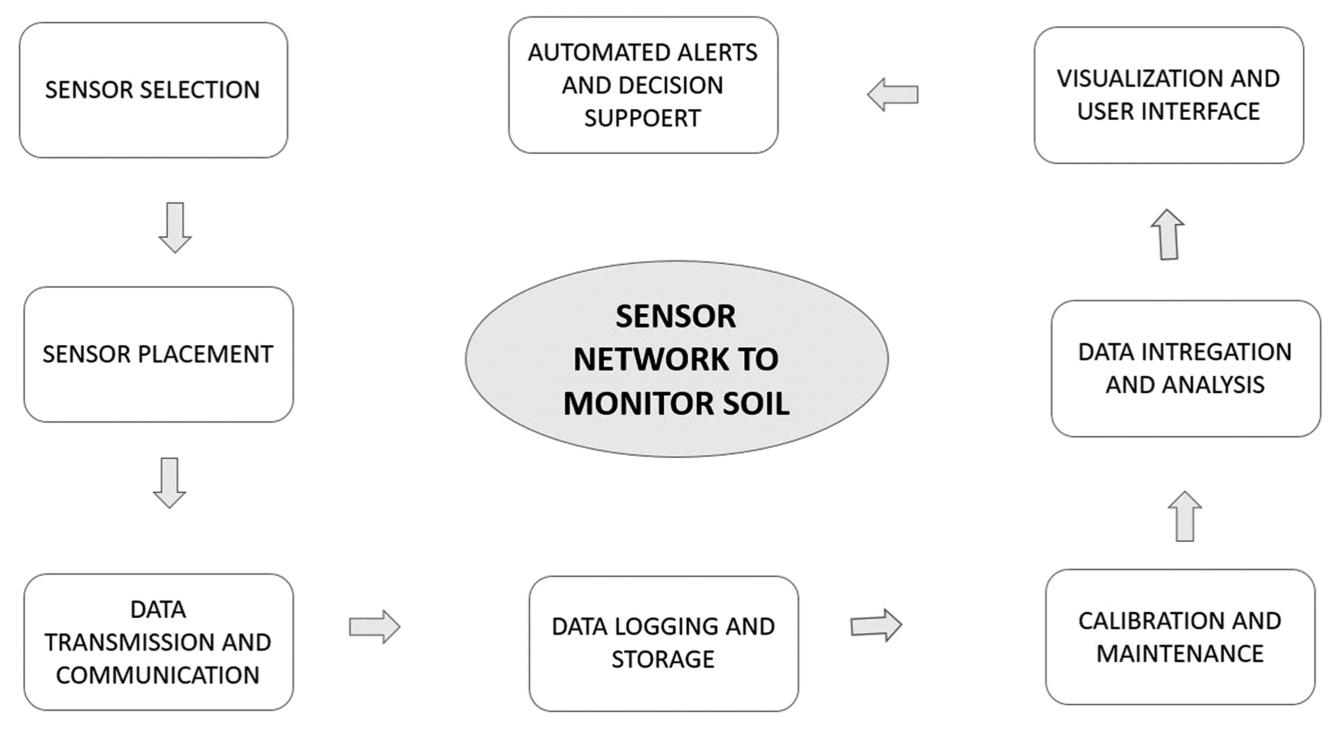
\includegraphics[height=0.6\textheight]{images/chap7_p7_1.jpeg}
        \caption{Hình 7.2: Sơ đồ Triển khai mạng cảm biến giám sát đất}
    \end{figure}
\end{frame}

\begin{frame}{Tối ưu hóa tưới tiêu: Hệ thống thông minh}
    \begin{columns}
        \begin{column}{0.5\textwidth}
            \begin{figure}[h]
                \centering
                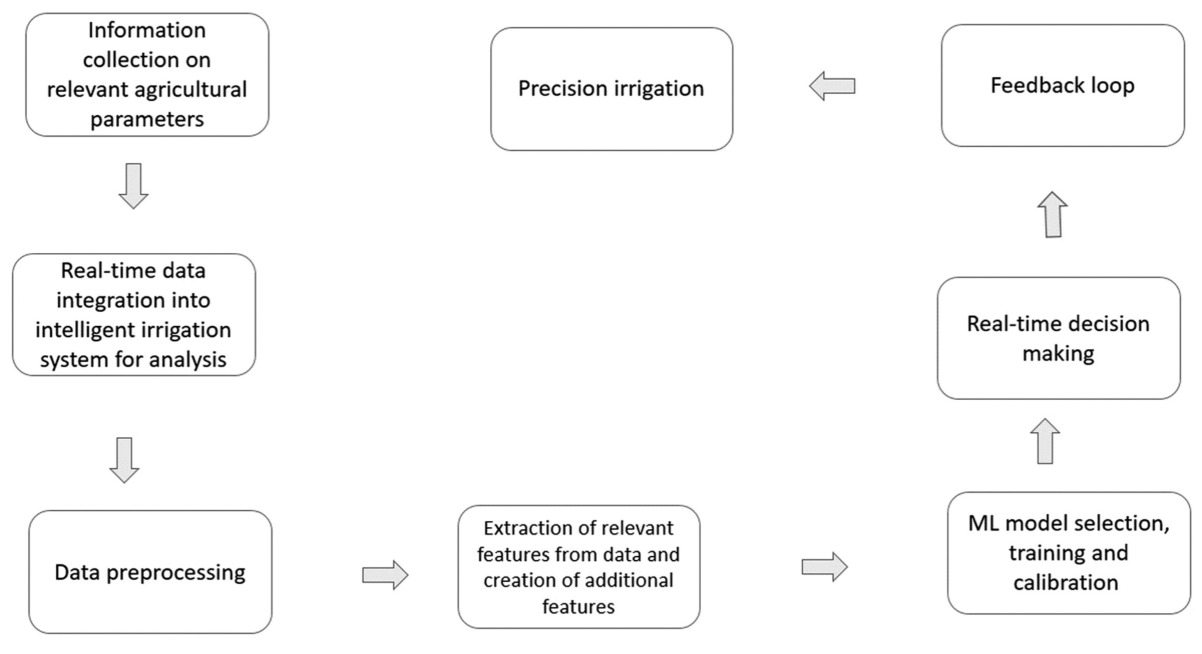
\includegraphics[width=0.9\textwidth]{images/chap7_p7_2.png}
                \caption{Hình 7.3: Hệ thống tưới tiêu thông minh}
            \end{figure}
        \end{column}
        \begin{column}{0.5\textwidth}
            \begin{figure}[h]
                \centering
                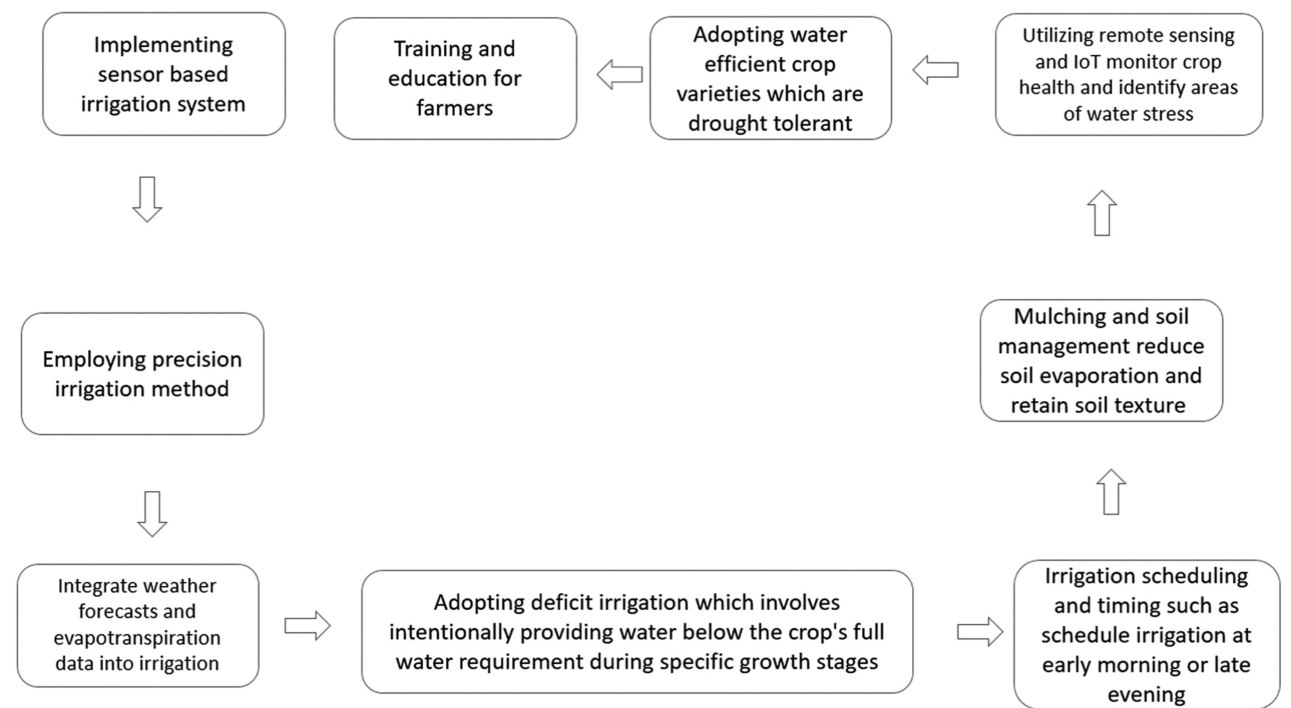
\includegraphics[width=0.9\textwidth]{images/chap7_p8_1.png}
                \caption{Hình 7.4: Cung cấp đủ nước cho cây trồng}
            \end{figure}
        \end{column}
    \end{columns}
    \vspace{0.3cm}
    $\rightarrow$ Thuật toán ML xử lý dữ liệu thời gian thực và tự động ra quyết định tưới nước chính xác, giảm lãng phí.
\end{frame}

\begin{frame}{Học tăng cường trong Tưới tiêu}
    \begin{figure}[h]
        \centering
        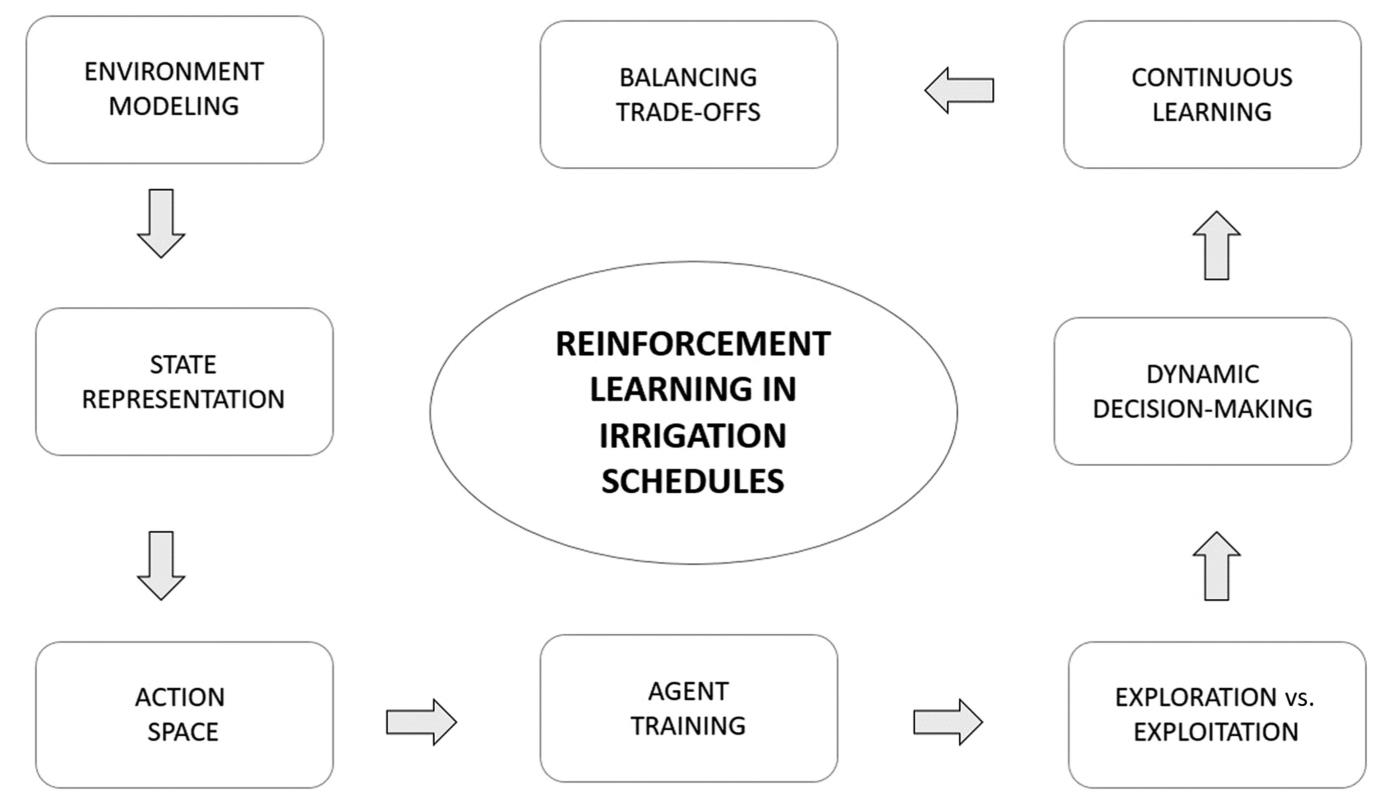
\includegraphics[height=0.6\textheight]{images/chap7_p9_1.jpeg}
        \caption{Hình 7.5: Điều chỉnh tự động lịch trình tưới tiêu (Học tăng cường)}
    \end{figure}
\end{frame}

\section{Quản lý vật nuôi}
\begin{frame}{Quản lý vật nuôi: Giám sát tự động}
    Giám sát sức khỏe, hành vi, và phúc lợi của vật nuôi bằng cảm biến (GPS, thẻ tai):
    \begin{figure}[h]
        \centering
        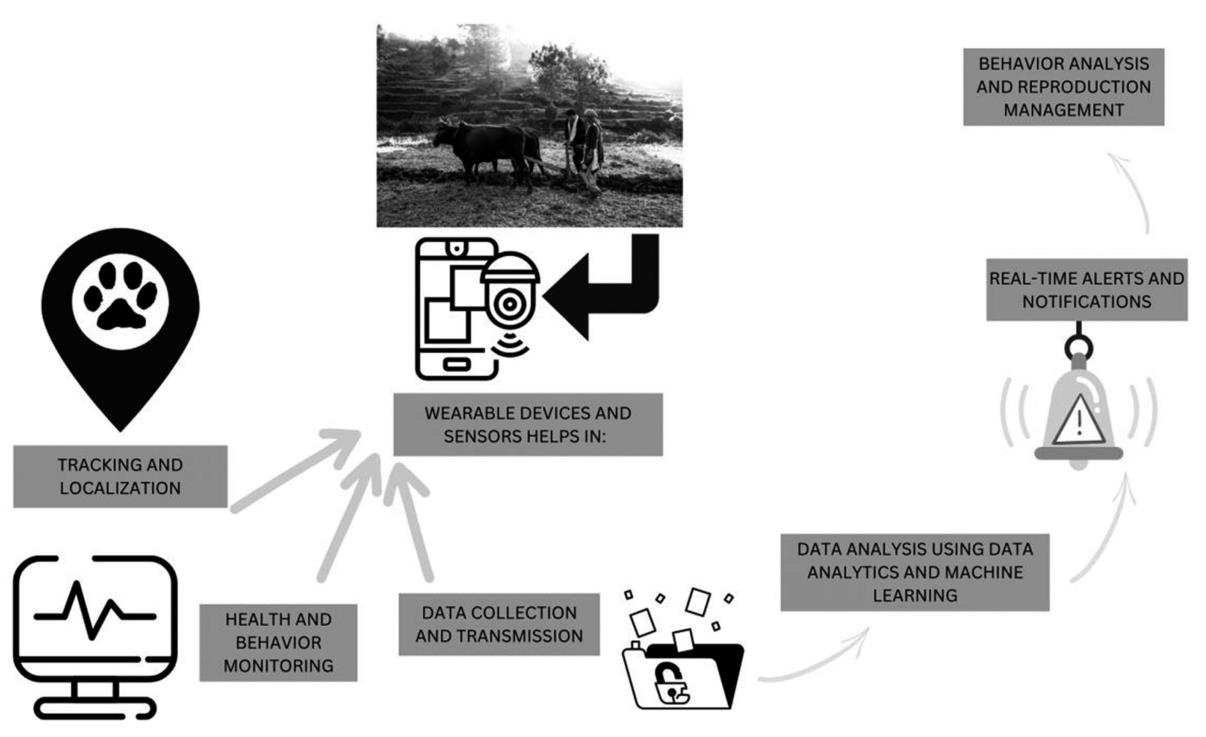
\includegraphics[height=0.55\textheight]{images/chap7_p10_1.jpeg}
        \caption{Hình 7.6: Hệ thống giám sát tự động bằng cảm biến và phân tích ML}
    \end{figure}
\end{frame}

\begin{frame}{Tác dụng của giám sát vật nuôi}
    \begin{itemize}
        \item \textbf{Theo dõi và Định vị}: Ngăn chặn đi lạc, quản lý khu vực chăn thả hiệu quả bằng GPS.
        \item \textbf{Sức khỏe \& Hành vi}: Phát hiện thói quen ăn uống bất thường, dấu hiệu căng thẳng hoặc bệnh tật.
        \item \textbf{Quản lý sinh sản}: Phát hiện hành vi động dục ở động vật cái để nhân giống đúng thời điểm.
        \item \textbf{Cảnh báo thời gian thực}: Nhận thông báo qua điện thoại để can thiệp y tế ngay lập tức.
    \end{itemize}
\end{frame}

\section{Tối ưu thức ăn chăn nuôi}
\begin{frame}{Tối ưu hóa thức ăn chăn nuôi bằng ML}
    Tạo ra các kế hoạch cho ăn được cá nhân hóa nhằm tối đa hóa năng suất (sữa, thịt) và giảm thiểu chi phí:
    \begin{enumerate}
        \item Thu thập dữ liệu (loài, giống, tuổi, cân nặng, tình trạng sinh lý).
        \item Đặt yêu cầu dinh dưỡng mục tiêu.
        \item Công thức hóa vấn đề thành bài toán ML (Tối ưu hóa đa mục tiêu).
        \item Huấn luyện mô hình (Hồi quy, Thuật toán di truyền) dựa trên hiệu suất lịch sử.
        \item Áp dụng và cập nhật công thức theo thời gian thực dựa trên sự sẵn có của nguyên liệu.
    \end{enumerate}
\end{frame}

\section{Kết luận}
\begin{frame}{Kết luận}
    \begin{block}{Chuyển đổi số trong Nông nghiệp}
        ML đang thay đổi diện mạo nông nghiệp thông qua các hệ thống dự báo năng suất, tưới tiêu thông minh, quản lý đất đai và tự động hóa giám sát vật nuôi.
    \end{block}
    
    \vspace{0.3cm}
    \textbf{Tầm nhìn}: 
    Khi rào cản về hạ tầng và giáo dục được giải quyết, AI/ML sẽ mở ra kỷ nguyên mới: **canh tác bền vững, nâng cao an ninh lương thực và bảo vệ sinh thái.**
\end{frame}

\begin{frame}
    \centering \Huge \textbf{Xin Cảm Ơn!}
\end{frame}

\end{document}
